\chapter{Verification} \label{chapt:verification}

% ==============================================================================
%
%                             image processing
%
% ==============================================================================
\section{Image Processing}
The image processing part was tested with an image from a street. The image was read in the C simulation and the Co simulation and filtered with the sobel algorithm and compared. As well as with the implemented IP-core filtered on the FPGA and compared to the two simulations. These verification steps are illustrated in the figure \ref{fig:ip_validation}. They must all provide the same result to ensure that the algorithm is correct. These three steps are in the following three chapters.

\begin{figure}[b!]
    \centering
    \begin{adjustbox}{width=0.5\textwidth}
        % \tikzsetnextfilename{system-overview}
\begin{tikzpicture}[
    rounded corners=0mm,
]
    %coordinates
    \coordinate (orig)      at (0,0);
    \coordinate (csim)      at (0,0);
    \coordinate (cosim)     at (2,-1.5);
    \coordinate (fpga)     at (-2,-1.5);


    %nodes
    \node[draw, fill=white, minimum width=3cm, minimum height=1cm, anchor=south, text width=2.8cm, align=center] (A) at (csim) {C Simulation};
    \node[draw, fill=white, minimum width=3cm, minimum height=1cm, anchor=south, text width=2.8cm, align=center] (B) at (cosim) {Co Simulation};
    \node[draw, fill=white, minimum width=3cm, minimum height=1cm, anchor=south, text width=2.8cm, align=center] (C) at (fpga) {FPGA Test};

    %path
    \path[draw,-{Latex[length=2.5mm]}] (A) -- (B);
    \path[draw,-{Latex[length=2.5mm]}] (B) -- (C);
    \path[draw,-{Latex[length=2.5mm]}] (C) -- (A);

\end{tikzpicture}
    \end{adjustbox}
    \caption{Verification flow of the Sobel filter}
    \label{fig:ip_validation}
\end{figure}

In a second step the synthesis of the algorithm is checked. The synthesis and implementation of the HLS is compared with the implementation on the FPGA. This verification is checked in chapter \ref{sec:synth}.

% ==============================================================================
%
%                             C Simulation
%
% ==============================================================================

\subsection{C Simulation} \label{sec:csim}
%%Eine Testbench für die Simulation muss vorhanden sein, um die Software auf dem PC zu testen.
% - Berechnete Pixel vergleichen?

The C simulation is the first step to test the algorithm. A C/C++ testbench must be available for this simulation. With Vivado HLS the algorithm can be simulated with the testbench.
The testbench is constructed in such a way that it reads an image and makes the image data available to the algorithm in the correct order. The algorithm processes the data and returns it back to the testbench. The testbench creates an image from the filtered data, which can be compared with the Co simulation and the FPGA test. Figure \ref{fig:orig_street} shows the original street image and figure \ref{fig:c_street0} represents the image filtered with the C/C++ code.


\begin{figure}[tb!]
\centering
    \begin{minipage}[b]{0.47\textwidth}
        \centering
        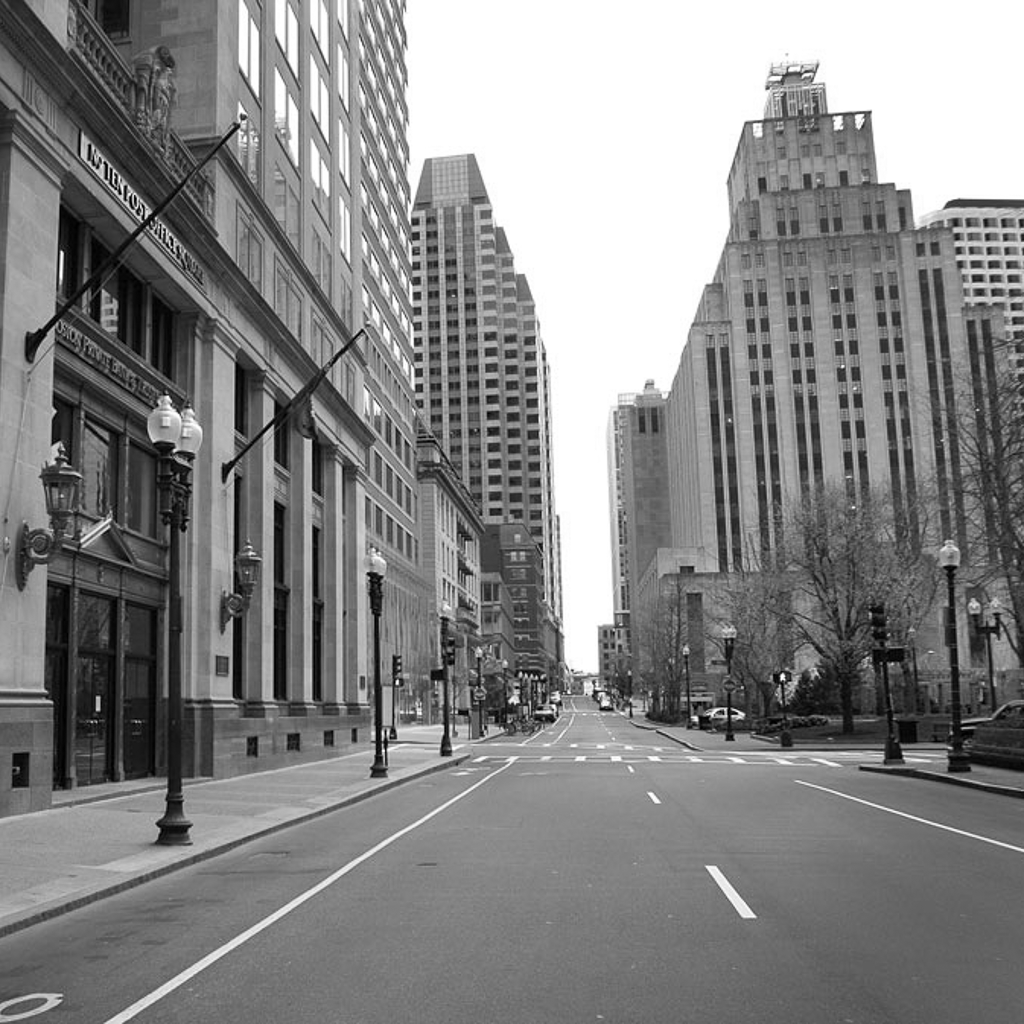
\includegraphics[width=\textwidth]{images/validation/street1024.png}
        \caption{Original Image}
        \label{fig:orig_street}
    \end{minipage}
\hspace{0.5cm}
    \begin{minipage}[b]{0.47\textwidth}
        \centering
        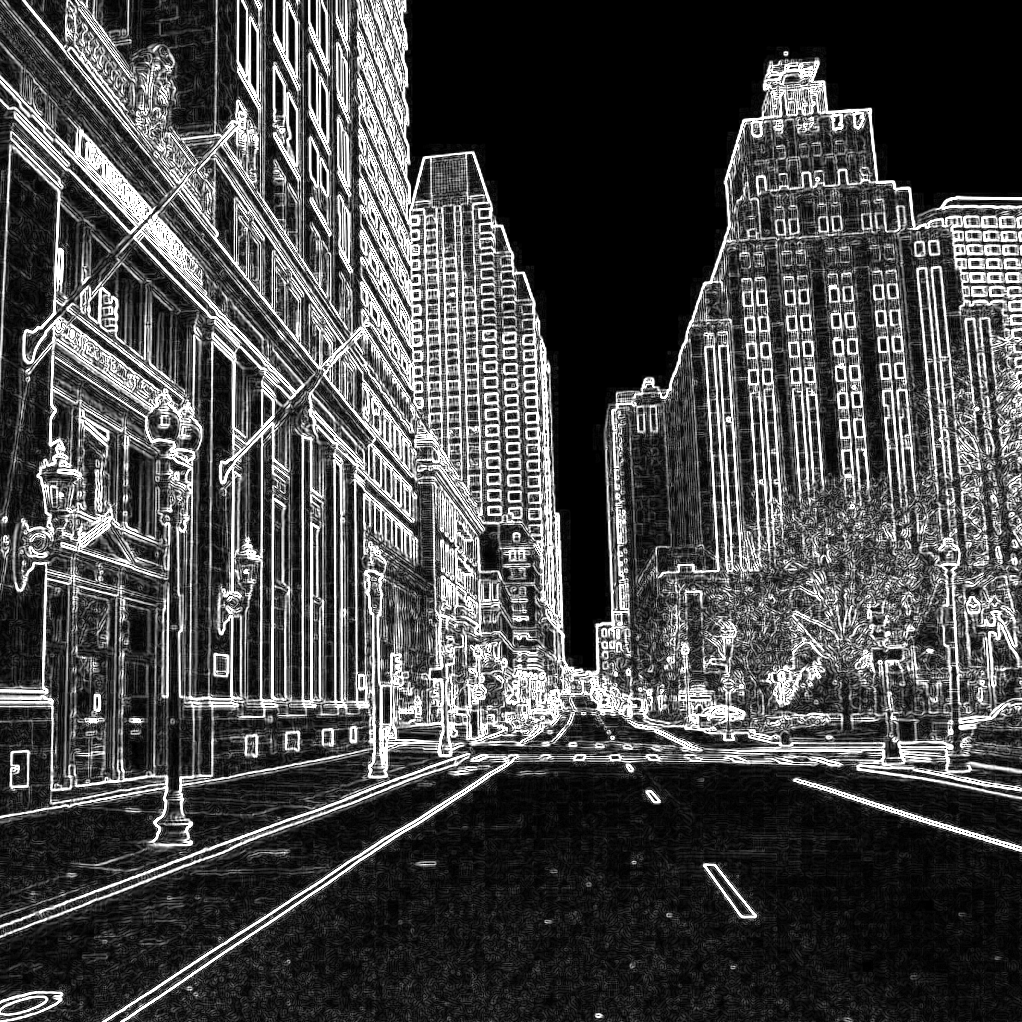
\includegraphics[width=\textwidth]{images/validation/c_street1024.png}
        \caption{C simulation Sobel image}
        \label{fig:c_street0}
    \end{minipage}
\end{figure}

% ==============================================================================
%
%                             Co Simulation
%
% ==============================================================================

\subsection{Co Simulation} \label{sec:cosim}
%%Der Code wird Hardwaremässig auf dem PC simuliert. Die C- und Co-Simulation müssen übereinstimmen
% - C Simulation mit Co-Siulation vergleichen
The Co simulation is the second step of the verification. This can be used to compare the C and Co simulation. The Co simulation generates the VHDL code from the algorithm.
In the Co Simulation, Vivado HLS extracts the data that the algorithm needs from the C testbench. The data is stored in files. This data is read by the generated RTL testbench and processed in VHDL code. This processed data is also stored in a file. This processed data is used to create the image that can be compared with the C simulation.

\subsubsection*{Comparison}
The image of the C simulation \ref{fig:c_street1} and the Co simulation \ref{fig:co_street0} are identical. The algorithm can be implemented in the FPGA and the third step of verification can be tested. \\

\begin{figure}[tb!]
\centering
    \begin{minipage}[b]{0.47\textwidth}
        \centering
        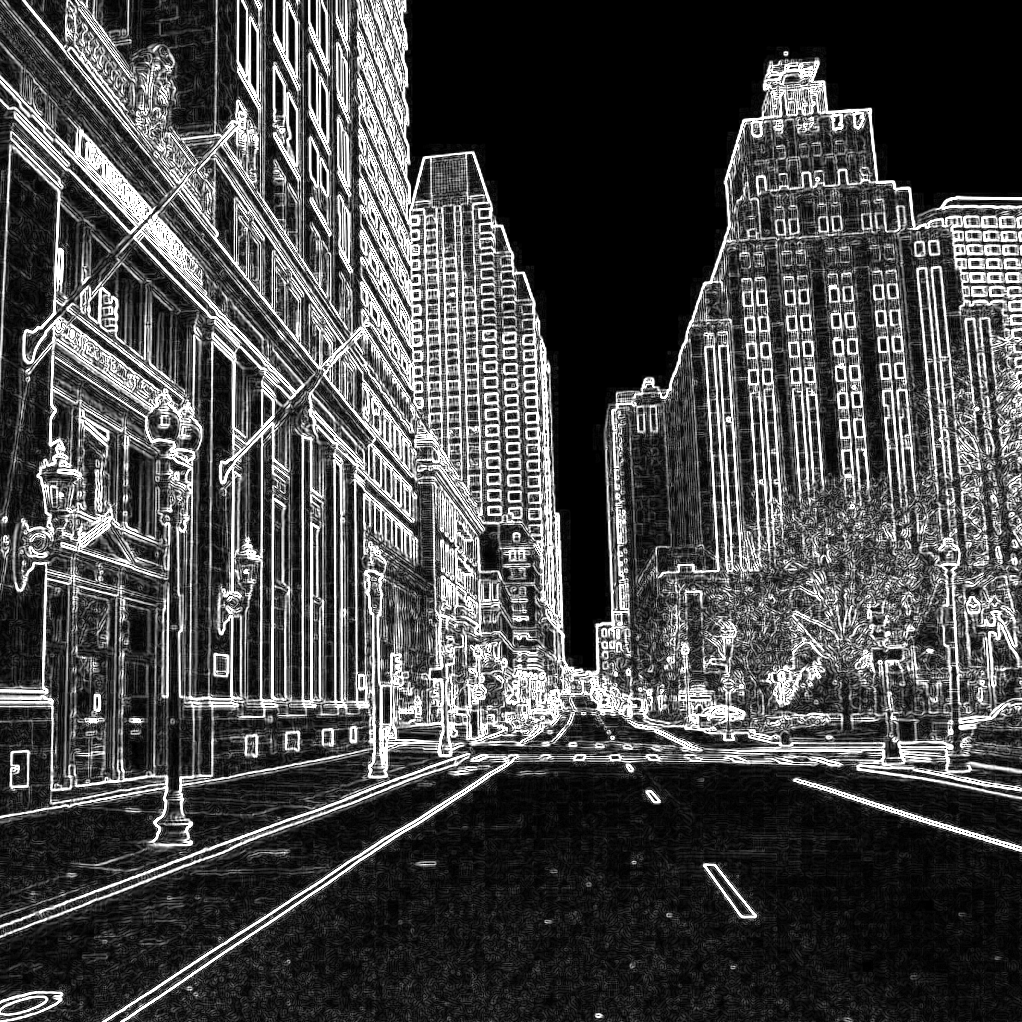
\includegraphics[width=\textwidth]{images/validation/c_street1024.png}
        \caption{C simulation Sobel image}
        \label{fig:c_street1}
    \end{minipage}
\hspace{0.5cm}
    \begin{minipage}[b]{0.47\textwidth}
        \centering
        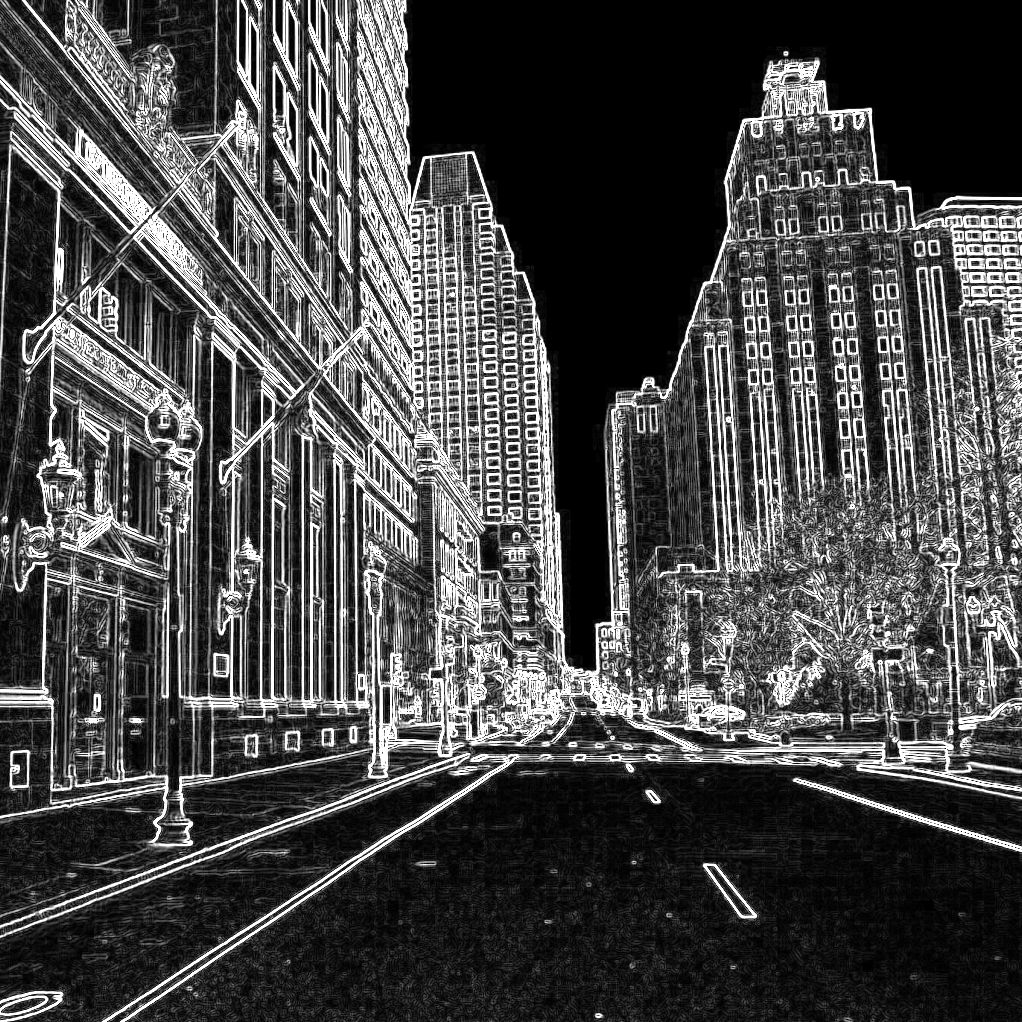
\includegraphics[width=\textwidth]{images/validation/co_street1024.png}
        \caption{Co simulation Sobel image}
        \label{fig:co_street0}
    \end{minipage}
\end{figure}

The two images in figures \ref{fig:c_street1} and \ref{fig:co_street0} were compared with \texttt{ImageMagick}. The mean square error (MSE) of these images were evaluated. The comparison in listing \ref{lst:comparison1} returned an MSE of 0, so the two images are identical.

\begin{minipage}{\linewidth}
\vspace{1ex}
    \begin{lstlisting}[
        style=ShellStyle, caption=C and Co Simulation image comparison, label=lst:comparison1
        ]
$ CMP='compare -verbose -metric MSE'
$ $CMP c_street1024.png co_street1024.png diff.png
Image: c_street1024.png
  Channel distortion: MSE
    gray: 0 (0)
    all: 0 (0)
\end{lstlisting}
\end{minipage}
\vspace{1ex}


% ==============================================================================
%
%                             FPGA Test
%
% ==============================================================================

\subsection{Test on FPGA} \label{sec:impl}
%%Der generierte IP-Core wird mittels JTAG-Interface getestet. Dafür ist eine Testbench nötig, welche Daten auf den FPGA schreibt und liest.
% Bild mit OpenCV sobel visuel vergleichen

The algorithm finally can be tested with the test on the FPGA. The result must match the C and the Co simulation.
In order to test the FPGA, a testbench was created with a TCL file for the FPGA. This testbench has basically the same style as the C testbench. It reads the image data from a file and sends it to the FPGA via JTAG. The IP core filters the data and sends it back to the PC via JTAG. On the PC, the filtered image can be generated from the image data and compared with the two other simulations.


\subsubsection*{Comparison}
The image of the FPGA test in figure  \ref{fig:fpga_street0} and the two other simulations (figure \ref{fig:c_street1} and figure \ref{fig:co_street1}) are identical. \\

\begin{figure}[tb!]
\centering
    \begin{minipage}[b]{0.47\textwidth}
        \centering
        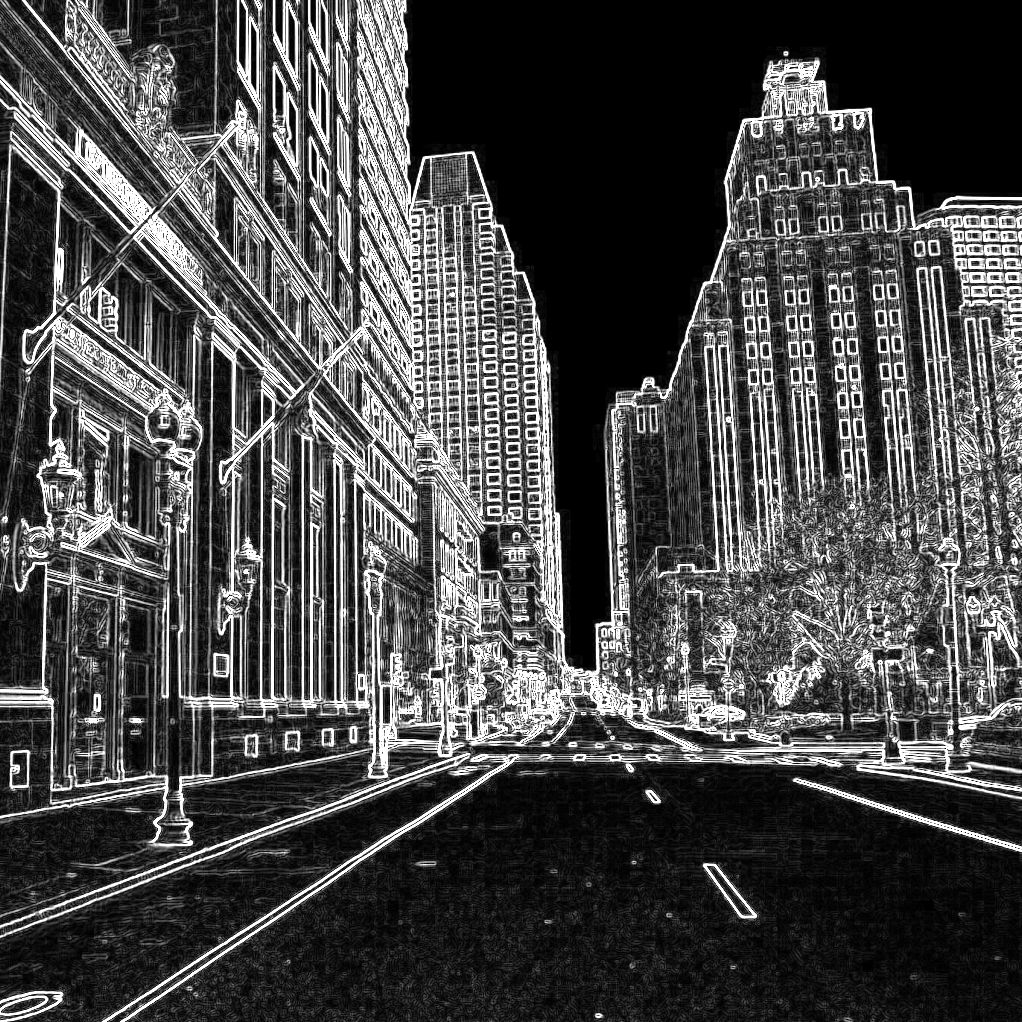
\includegraphics[width=\textwidth]{images/validation/co_street1024.png}
        \caption{Co simulation Sobel image}
        \label{fig:co_street1}
    \end{minipage}
\hspace{0.5cm}
    \begin{minipage}[b]{0.47\textwidth}
        \centering
        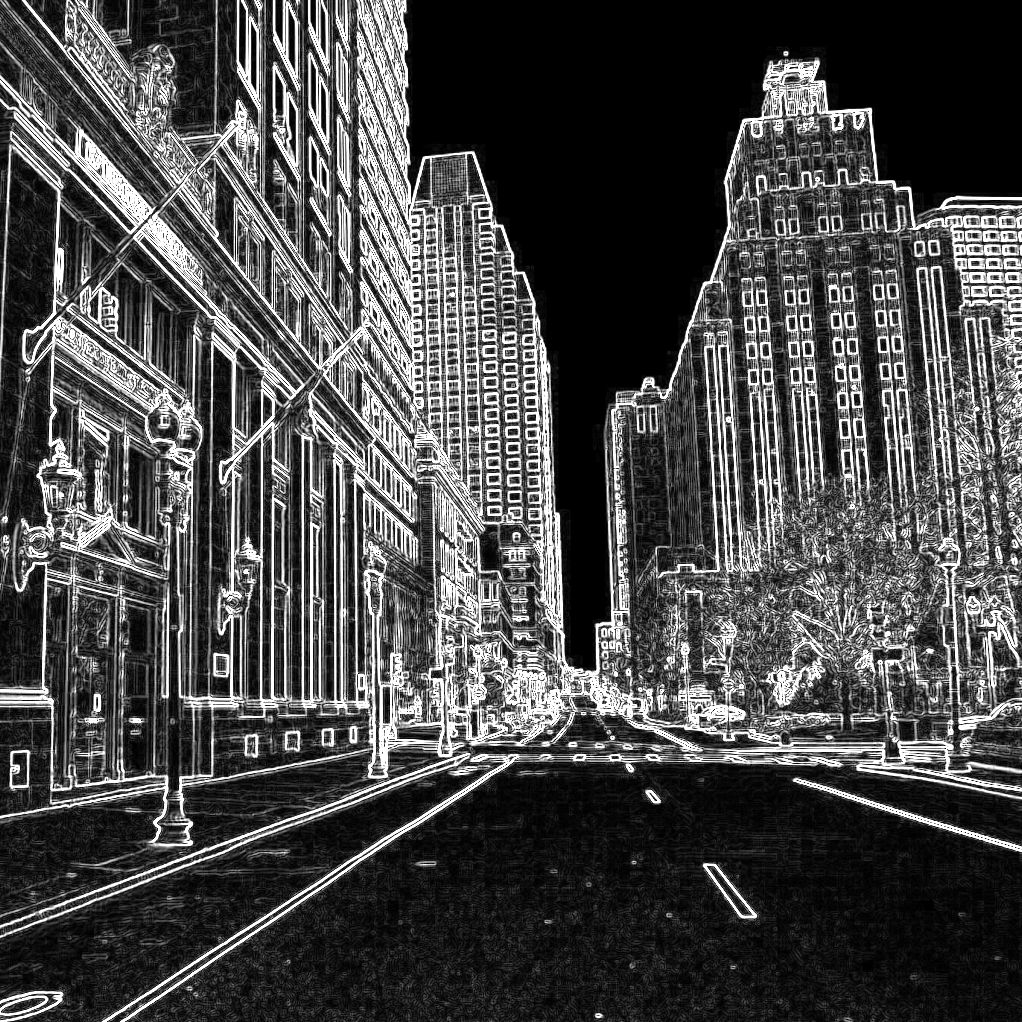
\includegraphics[width=\textwidth]{images/validation/fpga_sobel_street1024.png}
        \caption{FPGA test Sobel image}
        \label{fig:fpga_street0}
    \end{minipage}
\end{figure}

The two images in figure \ref{fig:co_street1} and \ref{fig:fpga_street0} were compared with \texttt{ImageMagick}. The mean square error (MSE) of these images were evaluated. The comparison in listing \ref{lst:comparison2} returned an MSE of 0, so the two images are identical. The algorithm has passed the validation and it can be said that the Sobel filter works on the hardware.

\begin{minipage}{\linewidth}
\vspace{1ex}
    \begin{lstlisting}[
        style=ShellStyle, caption=Co Simulation and FPGA test image comparison, label=lst:comparison2
        ]
$ CMP='compare -verbose -metric MSE'
$ $CMP co_street1024.png fpga_sobel_street1024.png diff.png
Image: co_street1024.png
  Channel distortion: MSE
    gray: 0 (0)
    all: 0 (0)
\end{lstlisting}
\end{minipage}
\vspace{1ex}



% ==============================================================================
%
%                             Synthesis
%
% ==============================================================================
\clearpage
\subsection{Synthesis} \label{sec:synth}
%%Der Code wird synthetisiert und kann analysiert werden. Daraus erhält man Informationen über die Latenz, Area, Timing, ...
% - Throughput, Latenz, Area, Timing von Hand bestimmen?
% - Analyse vergleichen und berechnen

The synthesis of the C/C++ code provides information on the throughput, latency and area of the design. This information can be compared with the implementation report of the IP core and later with the implemented IP core by Vivado HLx on the FPGA. 
The synthesis and implementation data can be read from a report file of Vivado HLS. To verify the data on the FPGA, a debug core was implemented on the FPGA and the clock cycles were measured. Triggered on the start and the done signal of the Sobel filter. The debugging can be seen in the figure \ref{fig:fpga_time}.

\begin{figure}[t!]
    \centering
    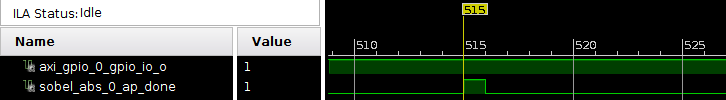
\includegraphics[width=\textwidth]{images/validation/fpga_time.png}
    \caption{Debugging window to measurement the clock cycles}
    \label{fig:fpga_time}
\end{figure}

\subsubsection*{Comparison}
The test results are listed in the table \ref{tab:synthesis}. The timing was set to 10ns for simulation and test. This resulted in the timing which could be achieved with regard to the critical paths. The latency is the same for every test and you get a throughput of 1 pixel per clock. This means 8 bits per clock cycle. The number of flip-flops and LUTs used after synthesis is much higher. This is to due the fact that the synthesized design is not yet optimized. \\

With a throughput of 1 pixel per clock and a timing of 10ns an image with 1500MPixel could be processed within 15 seconds with the Sobel filter.

\begin{equation}
    t = \frac{1500MPixel}{1 Pixel/Clk} \cdot 10ns = 15sec
    \label{eq:throughput}
\end{equation}

\begin{table}[h!]
    \centering
    \begin{tabular}{ l l l l }
        \toprule
         & Synthesis & Implementation & Debugging \\ 
        \midrule
        Timing achieved [ns] & 8.5 & 7 & 10 \\
        Latency [clock cycles] & 515 & 515 & 515 \\ 
        Throughput [Pixel / Clk] & 1  & 1 & 1 \\
        FF & 3451 & 964 & - \\ 
        LUT & 2512 & 1147 & - \\ 
        \bottomrule
    \end{tabular}
    \caption{Verification of the Synthesis}
    \label{tab:synthesis}
\end{table}

% ==============================================================================
%
%                             Communication
%
% ==============================================================================
\clearpage
\section{Communication}
The communication part of the project is tested using VHDL testbenches and
manual waveform verification. The subsequent sections are referring to the code
located under \path{fpga/hlx/cores/uft_stack_v1_0/} and the following paths are
relative to this location.

\subsection{HDL Testbench}
Each entity of the UFT stack is tested using a testbench. Most have a dedicated
testbench and few are tested in a top testbench. Table \ref{tab:ufttb} shows the
correspondence.

These testbenches stimulate the entity under test using input values whose output
results are known. The output is then inspected in a waveform viewer. In few
cases the testbench reads the output signals and verifies them automatically.
This would be the more reliable method but requires more time in designing the
testbenches.
\\

To generate UFT packets for testing the receiver, a program written in C is used
to assemble the packets. The packet analyzer WireShark is used to capture the
entire Ethernet frame and then store the byte sequence in a file. For example
the file \path{bench/uft_cmd_tcid_0c_nseq_1.txt} is a byte sequence in ASCII
containing the Ethernet, IP, UDP and UFT header for a UFT FTS command with
transaction ID \texttt{0x0c} and NSEQ \texttt{1}. This file is then read by the
\texttt{file2axistream} procedure in \texttt{uft\_top\_tb} and converted to a
corresponding AXI stream coming from the Tri-Mode Ethernet MAC. Listing 
\ref{lst:file2axistream} shows said procedure.

\begin{table}[h!]
    \centering
    \begin{tabular}{l l}
        \toprule
        Entity & Verified in \\
        \midrule

        \texttt{fifo\_32i\_8o} & \texttt{fifo\_32i\_8o\_tb} \\
        \texttt{fifo\_8i\_32o} & \texttt{fifo\_8i\_32o\_tb} \\
        \texttt{simple\_fifo} & \texttt{fifo\_32i\_8o\_tb} and 
        \texttt{fifo\_8i\_32o\_tb} \\
        \texttt{uft\_pkg} & - \\
        \texttt{uft\_rx} & \texttt{uft\_top\_tb} \\
        \texttt{uft\_rx\_mem\_ctl} & \texttt{uft\_top\_tb} \\
        \texttt{uft\_top} & \texttt{uft\_top\_tb} \\
        \texttt{uft\_tx} & \texttt{uft\_tx\_tb} \\
        \texttt{uft\_tx\_arbiter} & \texttt{uft\_tx\_tb} \\
        \texttt{uft\_tx\_cmd\_assembler} & \texttt{uft\_tx\_cmd\_assembler\_tb} \\
        \texttt{uft\_tx\_ctrl} & \texttt{uft\_tx\_ctrl\_tb} \\
        \texttt{uft\_tx\_data\_assembler} & \texttt{uft\_tx\_data\_assembler\_tb} \\
        \bottomrule
    \end{tabular}
    \caption{UFT Stack testbench assignment}
    \label{tab:ufttb}
\end{table}

\clearpage
\begin{minipage}{\linewidth}
    \begin{lstlisting}[
        style=VHDLStyle, 
        caption=Procedure file2axistream to generate AXI stream data, 
        label=lst:file2axistream
        ]
------------------------------------------------------------------------
-- Sends a file via axi stream
-- Data in file must be 1 byte per line, hex without 0x
-- ---------------------------------------------------------------------
procedure file2axistream ( fname : in string ) is
------------------------------------------------------------------------
    file fd             : text;
    variable iline      : line;
    variable byte       : std_logic_vector(7 downto 0);
    variable nbytes     : integer := 0;
begin
    file_open(fd, fname, read_mode);
    -- Count numbers of bytes in file
    while not endfile(fd) loop
        readline (fd, iline);
        nbytes := nbytes + 1;
    end loop;
    file_close(fd); file_open(fd, fname, read_mode);
    mac_rx_tlast <= '0';
    -- output the bytes to the axi stream
    while not endfile(fd) loop
        if mac_rx_tready = '1' then
            mac_rx_tvalid <= '1';
            if nbytes = 1 then mac_rx_tlast <= '1'; end if;
            readline (fd, iline); hread(iline,byte);
            mac_rx_tdata <= byte;
            nbytes := nbytes - 1;
        end if;
        waitfor(1); -- 1 clock pereiod
    end loop;
    mac_rx_tvalid <= '0';
    mac_rx_tlast <= '0';
    waitfor(1); -- 1 clock pereiod
end procedure file2axistream;\end{lstlisting}
\end{minipage}

\clearpage
Figure \ref{fig:file2axistream} shows the beginning waveform of the file 
\path{bench/uft_cmd_tcid_0c_nseq_1.txt} converted to a AXI Stream using the 
\texttt{file2axistream} procedure.
\\

\begin{figure}[t!]
    \centering
    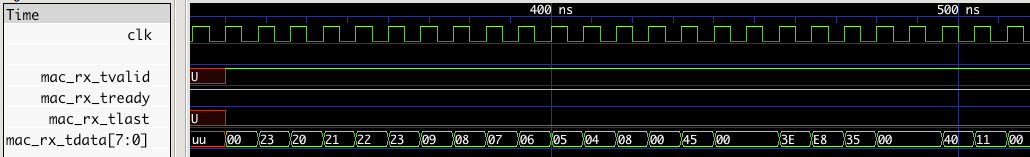
\includegraphics[width=\textwidth] {images/validation/file2axistream.png}
    \caption{Output of file2axistream}
    \label{fig:file2axistream}
\end{figure}

To test the transmitting part of the UFT stack the AXI stream coming from the
UDP IP Stack is stored in an ASCII file similar to the procedure used in listing
\ref{lst:file2axistream}. The process \texttt{p\_axi\_stream\_check} in the
entity \texttt{uft\_top\_tb} listens on the AXI Stream and stores the data in an
output file. For each transaction a new file is written. Running test 
\texttt{t10} in \texttt{uft\_top\_tb} with \texttt{tx\_data\_size} set to 1025
yields four log files in \path{../../build/ghdl}:

\vspace{1em}
\begin{minipage}{\linewidth}
    \begin{lstlisting}[
        style=ShellStyle, 
        ]
build/ghdl/axi_stream_res_0.log
build/ghdl/axi_stream_res_1.log
build/ghdl/axi_stream_res_2.log
build/ghdl/axi_stream_res_3.log\end{lstlisting}
\end{minipage}
\vspace{1em}

Each file corresponds to an Ethernet frame coming from the UDP IP Stack. 
\texttt{res\_0} is an ARP request to get the MAC address of the destination.
\texttt{res\_1} is the UFT FTS command and \texttt{res\_2} and \texttt{res\_3}
the two UFT data packets. To validate the UFT packets the data is copied into an
Excel sheet that analyzes the packets. Figure \ref{fig:uftcheck} shows the
output.

\begin{figure}[b!]
    \centering
    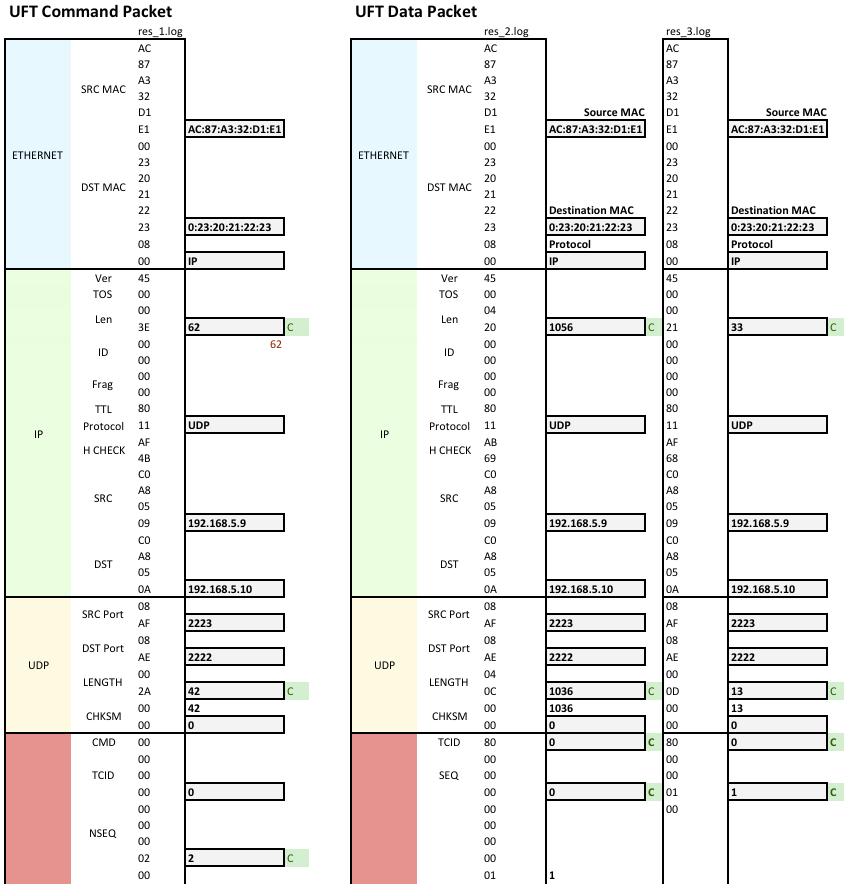
\includegraphics[width=\textwidth] {images/validation/uftcheck.png}
    \caption{\url{UFT Protocol Checker.xlsx} with output of test 10 of
    uft\_top\_tb}
    \label{fig:uftcheck}
\end{figure}

% ==============================================================================
%
%                             PC to FPGA Communication
%
% ==============================================================================
\clearpage
\subsection{PC to FPGA Communication}
After the UFT stack is verified in simulation it is implemented in hardware. To
test the functionality the following tools are used:
\begin{itemize}
    \item tcl script \url{fpga/hlx/projects/diip/testbench/jtag_axi.tcl} to read
    and write to the FPGA block memory and set transaction sizes
    \item \url{sw/udp_test/sender} and \url{sw/udp_test/receiver} to send and
    receive files using UFT
    \item WireShark network protocol analyzer \cite{wireshark}
\end{itemize}

In the subsequent tests the AC701 evaluation kit is directly connected to an
Apple Mac Book Pro with a Cat.5e cable and Ethernet to lightning adapter. Table
\ref{tab:ufttestconf} shows the connection setup.
\\
\begin{table}[b!]
    \centering
    \begin{tabular}{l l l}
        \toprule
        {} & Computer & FPGA \\
        \midrule
        IP address & 192.168.50.10 & 192.168.50.9 \\
        Hardware address & {} & 00:23:20:21:22:23 \\
        UFT send port & 42042 & 2222 \\
        UFT receive port & 2222 & 42042 \\ 
        \bottomrule
    \end{tabular}
    \caption{UFT test setup}
    \label{tab:ufttestconf}
\end{table}

The first test is to send a file from the computer to the FPGA. A text file
named \url{testfile.txt} containing ASCII data is sent from the computer and
the FPGA decodes the UFT protocol and stores the file at the memory location
\texttt{0x0800\_0000}. A block memory is configured at this address to store the
data. To verify a successful transmission the Xilinx JTAG to AXI Master IP core
is used. It allows read and writes on the AXI Master bus through the JTAG
connection to the computer. The necessary tcl commands are defined in 
\url{jtag_axi.tcl}. Running the command \texttt{run\_hw\_axi rt} reads eight
data words from the block memory (one data word equals four data bytes on the
32 bit data bus). Issuing the command after configuring the FPGA returns all
zeros.

% TCL BRAM read
\vspace{1ex}
    \begin{lstlisting}[
        style=ShellStyle, 
        ]
Vivado% run_hw_axi rt
INFO: [Labtoolstcl 44-481] READ DATA is: 
    0000000000000000000000000000000000000000000000000000000000000000
\end{lstlisting}
\vspace{1ex}

Then the UFT file transfer is started on the computer using the \texttt{sender}
program with the FPGA IP address and the input file as argument. The file is
2.5KB in size so it will be sent in two data packets after the start command
packet is sent.

% UFT send
\vspace{1ex}
    \begin{lstlisting}[
        style=ShellStyle, 
        ]
$ ./sender 192.168.5.9 testfile.txt
UFT Sender demo
\end{lstlisting}
\vspace{1ex}

Now that the file is sent to the FPGA the block memory read transaction is
issued again and now returns data in hex format.

% TCL BRAM read
\vspace{1ex}
    \begin{lstlisting}[
        style=ShellStyle, 
        ]
Vivado% run_hw_axi rt
INFO: [Labtoolstcl 44-481] READ DATA is: 
    69206d65726f4c0a0a2e68616f4e20646e61206e614a20736920736968542021
\end{lstlisting}
\vspace{1ex}

Converting the hex data to ASCII, taking the last line and reversing the byte
order \footnote{the read transaction outputs the highest address first}
returns the first line of the textfile that was sent to the FPGA. This is proof
of a successful file transmission.

% Verify
\vspace{1ex}
    \begin{lstlisting}[
        style=ShellStyle, 
        ]
$ IN=69206d65726f4c0a0a2e68616f4e20646e61206e614a20736920736968542021
$ echo $IN | xxd -r -p | tail -n1 | rev
! This is Jan and Noah.
$ cat testfile.txt | head -n1
! This is Jan and Noah.
\end{lstlisting}
\vspace{1ex}

To debug the transmission, data communication on the computer's network
interface is captured using the network protocol analyzer WireShark. Figure 
\ref{fig:wiresharksend} shows a screenshot of the data capture. Frame 45 and 46
are the ARP request coming from the computer, asking for the hardware address of
the FPGA. Frame 47 is the UFT file transfer start command and frame 48 through
49 data packets one and two.

\begin{figure}[b!]
    \centering
    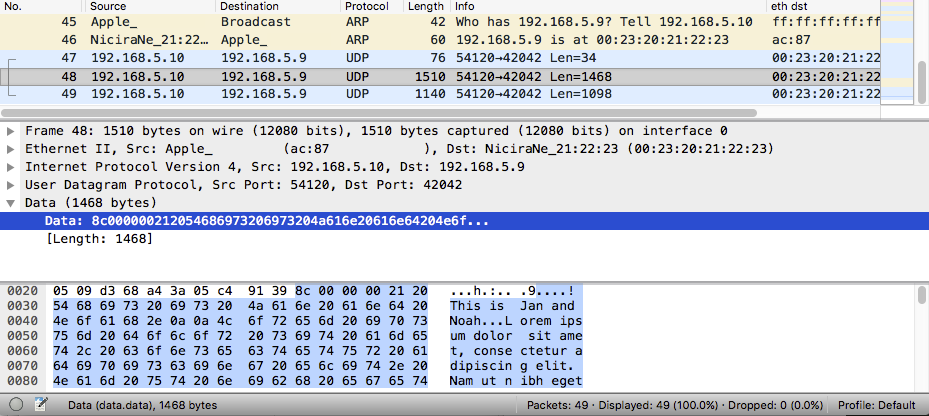
\includegraphics[width=\textwidth] {images/validation/wiresharksend.png}
    \caption{Ethernet capture of UFT send}
    \label{fig:wiresharksend}
\end{figure}

% ==============================================================================
%
%                             FPGA to PC Communication
%
% ==============================================================================
\clearpage
\subsection{FPGA to PC Communication}
Now that the file is sent to the FPGA and stored in block memory it can be sent
back to the computer. The UFT stack requires three input signals to start a file
transmission (see table \ref{tab:ufttxsig}). \texttt{dat\_src\_addr} is
hardwired to the address \texttt{0x0800\_0000}, the same as the UFT receiver.
The \texttt{data\_size} vector is connected to a AXI GPIO and can be set using
the same AXI write transaction used to write to block memory. Finally the
\texttt{tx\_start} signal is connected to a button on the evaluation kit
\footnote{a debouncer and impulse generator are connected between the pin and
the \texttt{tx\_start} signal}. 
\\

First, the UFT data size is set to 1MB by issuing the command 
\texttt{run\_hw\_axi sz1M} defined in \url{jtag_axi.tcl}.

% run_hw_axi sz1M
\vspace{1ex}
    \begin{lstlisting}[
        style=ShellStyle, 
        ]
Vivado% run_hw_axi sz1M
INFO: [Labtoolstcl 44-481] WRITE DATA is: 0010_0000
\end{lstlisting}
\vspace{1ex}

Now the UFT receiver is started on the computer using the \texttt{receiver}
program with the output file as argument. It listens for incoming UFT transfers,
decodes the packets, reassembles the data and writes it to the output file.
After the transfer is complete the elapsed time and the average
transfer speed is printed.

% run_hw_axi sz1M
\vspace{1ex}
    \begin{lstlisting}[
        style=TextStyle, 
        ]
$ ./receiver hifpga.bin
UFT Receiver demo
Waiting for data...
start writing file
time elapsed: 111939us Speed: 8.933 MB/s
\end{lstlisting}
\vspace{1ex}

To verify successful transmission the first line of the output file and the
first file of the test file are shown. The match indicates a valid transmission.

% verify
\vspace{1ex}
    \begin{lstlisting}[
        style=ShellStyle, 
        ]
$ cat hifpga.bin | head -n1
! This is Jan and Noah.
$ cat testfile.txt | head -n1
! This is Jan and Noah.
\end{lstlisting}
\vspace{1ex}

The data capture on the network connection captured 1025 frames. A 1MB file is
split into 1024 frames of 1024 bytes plus the start packet makes 1025 frames.
The incrementing sequence number can also be observed. Figure 
\ref{fig:wiresharkreceive} shows the UFT file reception.
\\

\begin{figure}[b!]
    \centering
    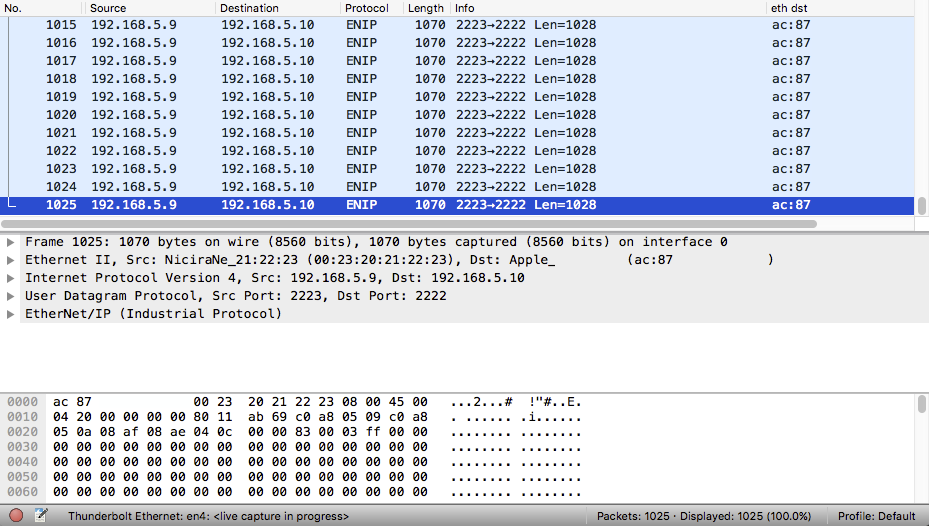
\includegraphics[width=\textwidth] {images/validation/wiresharkreceive.png}
    \caption{Ethernet capture of UFT receive}
    \label{fig:wiresharkreceive}
\end{figure}

The measured transfer speed of 8.93 MB/s is very close to the theoretical
maximum speed for 1024 byte data payload with 100$\mu s$ of 9.03 MB/s
calculated in appendix \ref{app:uftcalc}.

% \clearpage
% \subsection{Synthesis and Implementation Reports}
% Durch diese Reports kann sichergestellt werden, dass keine unnotigen Latches
% erstellt werden, kein Speicher verschwendet wird...


% ==============================================================================
%
%                             Complete System
%
% ==============================================================================
% \section{Complete System}
% An das Gesamtsystem werden Bilder gesendet, verarbeitet und wieder empfangen. 
% Dieselben Bilder werden mit einem C-Programm verarbeitet und danach verglichen.
